\section{Implementations}

% Don't draw any conclusions!
% - E.g. stop after saying that the "nested iterations" exception came up!
% - Conclusions belong to the Results/Conclusion sections

This section discusses our attempts at implementing the different approaches
described in section \ref{sec:approaches}. While we won't go over every single
line of our code, we will still give detailed insight into our implementations
in this section.

\subsection{Delta Iterations}

\subsection{Exploiting Mahout's LanczosSolver}


% Loop-Based Implementation
% =========================

\subsection{Loop-Based Implementation}

The loop-based approach discussed in section \ref{ssec:loop_approach} is
actually the one we started implementing first. The basic idea here was to
model the data flow of a single iteration step in Flink and and to implement
the actual iterations using ordinary Java loops. Our first step was to identify
the different modules we would have to develop in order to build a solid
foundation that we could implement the Lanczos algorithm on. The goal here was
not only to make the algorithm's implementation possible, but to provide an API
for ourselves that would make it convenient as well.

% High-Level Project Structure
% ----------------------------

\begin{figure}[h]
	\centering
	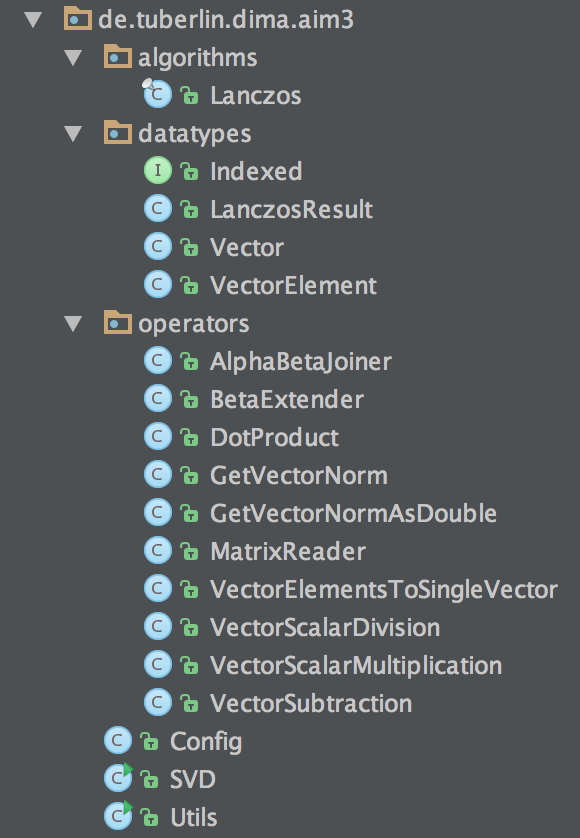
\includegraphics[scale=0.5]{images/loop_approach_project_structure}
    \caption{Core project structure of the loop-based implementation}
	\label{fig:loop_project_structure}
\end{figure}

Figure \ref{fig:loop_project_structure} shows the core project structure of our
loop-based implementation. On the top level, it consists of general
\texttt{Config} and \texttt{Utils} classes that contain configuration
parameters and utility functions, respectively. The \texttt{SVD} class acts as
the entry point to the program. Except for some pre- and post-processing, it
basically just invokes the Lanczos algorithm on an input matrix. The
interesting parts of the program are divided into the three sub-packages
\textit{algorithms}, \textit{datatypes} and \textit{operators}. As the
\textit{algorithms} package should be self-explanatory, we will only explain
the general ideas behind the \textit{datatypes} and  \textit{operators}
packages at this point. On that basis, we will then give a lower-level
description of our Lanczos implementation.

% Custom Datatypes
% ----------------

\subsubsection{Custom Datatypes}
\label{ssec:custom_datatypes}

As stated earlier, we aimed for a convenient internal API that would make large
parts of the implementation relatively comfortable for us by hiding
implementation details and by providing powerful abstractions for various kinds
of operations. To achieve this, we developed some custom data types that
provide all the mathematical operations we needed in a convenient way. They can
be found in the \textit{datatypes} package.

% Vector Class
% ------------

The main type of calculation needed in the Lanczos algorithm is vector algebra,
which is why the \texttt{Vector} class is the most verbose and probably one of
the most interesting classes in the project. One step of the Lanczos algorithm
is the multiplication of a matrix by a vector. But as a matrix can be seen as a
list of vectors and as we would have to split the matrix into its row vectors
in order to run this calculation in parallel anyway, we figured we wouldn't
have to implement a separate matrix class.

\begin{lstlisting}[label=lst:vector_usage,captionpos=b,caption=Example use of
the \texttt{Vector} class]
List<Double> v1Elements;
// (Fill the list with 3 vector elements)
Vector v1 = new Vector(v1Elements);
Vector v2 = new Vector.getRandomVector(3, 5); // 3 elements, norm = 5

double v1Norm     = v1.norm();     // L2 norm by default
Vector v1Scaled   = v1.scaleTo(1); // Scale v1 to norm 1
Vector difference = v1.minus(v2);
double dotProduct = v1.dot(v2);
Vector v1Doubled  = v1.times(2);
Vector v2Halved   = v2.divideBy(2);
\end{lstlisting}

Internally, the \texttt{Vector} class simply uses an ordinary Java list of
\texttt{Double} values to store its elements. The class allows new vector
instances to be constructed from a list of elements, from a Java map containing
elements mapped to their indices or by creating a copy of an existing vector.
It also provides static methods for constructing new zero vectors or random
vectors of arbitrary sizes. As for the actual algebra, the \texttt{Vector}
class contains instance methods for calculating a vector's norm, scaling a
vector to any target norm, subtracting one vector from another, building the
dot product of two vectors and multiplying or subtracting a vector by a scalar.
Listing \ref{lst:vector_usage} demonstrates usage of the \texttt{Vector} class
for convenient vector calculations.

% Other Datatypes
% ---------------

Compared to the vector type, the other custom data types are less important and
less interesting. The \texttt{VectorElement} class represents a value that has
an index of some sort, for example an index indicating the value's position in
a vector, but it doesn't implement any algebraic operations on that value.
Because the Lanczos algorithm's final result are two matrices, we wanted to
have a way of returning two matrices from a method, which we solved by wrapping
those two matrices inside the \texttt{LanczosResult} class.

% Custom Flink Operators
% ----------------------

\subsubsection{Custom Flink Operators}
\label{ssec:custom_operators}

Since Flink operates solely on data sets, one has to implement a Flink
program's data flow by defining custom operators and then invoking those
operators on data sets representing the relevant data. This is exactly the
purpose of the modules in our \textit{operators} package. Some of these modules
do calculations on vectors and scalar values, while others only transform
existing data from one form into another.

The operators \texttt{GetVectorNorm}, \texttt{GetVectorNormAsDouble},
\texttt{VectorScalarDivision}, \texttt{DotProduct},
\texttt{VectorScalarMultiplication} and \texttt{VectorScalarSubtraction} are
basically just wrapper classes that allow all the vector operations described
in section \ref{ssec:custom_datatypes} to be invoked on data sets in parallel
(more or less). This is where our custom vector class comes in handy, because
instead of manually working with instances of Java lists or Flink's tuple data
types to perform the necessary calculations, these operators can simply use our
vector API without having to know how the algebraic operations they use are
actually implemented.

\begin{lstlisting}[label=lst:vector_scalar_multiplication,captionpos=b,caption
=Implementation of the custom operator for vector-scalar multiplication]
// (Package definition + imports)

public class VectorScalarMultiplication
    extends RichGroupReduceFunction<Vector, Vector> {
    
  public void reduce(Iterable<Vector> vectors, Collector<Vector> out) {
    double scalar = getRuntimeContext()
                      .<VectorElement>getBroadcastVariable("scalar")
                      .get(0).getValue();
    vectors.forEach(vector -> out.collect(vector.times(scalar)));
  }
}
\end{lstlisting}

For example, our custom operator for vector-scalar multiplication, which
extends Flink's \texttt{RichGroupReduceFunction} and is shown in listing
\ref{lst:vector_scalar_multiplication}, simply uses our vector API's
\texttt{times()} method to calculate and emit the products of a single
broadcasted scalar value with all the vectors contained in the data set the
operator is invoked on. Thanks to the effort initially spent on developing a
custom vector type, we were able to implement most of the Flink operators we
needed very easily.

\subsubsection{Lanczos Algorithm}

The actual loop-based implementation of the Lanczos algorithm is contained in
the \texttt{Lanczos} class in the \textit{algorithms} package. It is mainly
based on the english Wikipedia article on the algorithm [5] as well as on the
algorithm's implementation in the Mahout machine learning library [3]. Listing
\ref{lst:lanczos} shows a pseudo code version of our implementation. Compared
to our actual Java implementation, this version is heavily simplified as it
leaves out many intermediate steps that are necessary when taking this
approach. In this listing an arrow from right to left stands for an assignment,
so for example \texttt{x <-- 42} means that the value 42 gets assigned to
\texttt{x}. Additionally, brackets after a data set name indicate read or write
access to the element in the data set whose index is equal to the value
specified in the brackets. For example \texttt{y[4]} would return the element
in data set \texttt{y} whose index is 4 and \texttt{y[2] <-- 1337} would store
the value 1337 in the data set \texttt{y} at index 2. Comments in parentheses
indicate parts of our implementation that have been left out for the sake of
simplicity.

\begin{lstlisting}[label=lst:lanczos,captionpos=b,caption=Pseudo code of our
loop-based Lanczos algorithm implementation (simplified)]
class Lanczos {
  process(A, m) {
    a <-- empty data set of scalar values
    b <-- empty data set of scalar values
    v <-- empty data set of vectors
    w <-- empty data set of vectors
    
    b[1] <-- 0
    v[0] <-- 0
    v[1] <-- random vector with norm 1
    
    for (j = 1...m-1) {
      w[j] <-- A.rowVectors().each(row -> row.dot(v[j]))
      // (Mahout style scaling of w[j])
      
      a[j] <-- w[j].dot(v[j])
      w[j] <-- w[j] - v[j].times(a[j]) - v[j-1].times(b[j])
      
      // (Orthogonalization)
      
      b[j+1] <-- w[j].norm()
      v[j+1] <-- w[j].divideBy(b[j+1])
    }
    
    w[m] <-- A.rowVectors().each(row -> row.dot(v[m]))
    a[m] <-- w[m].dot(v[m])
    
    tridiag = constructTridiagonalMatrix(a, b)
    
    return (tridiag, v)
  }
}
\end{lstlisting}

Within the main loop, our implementation uses a lot of intermediate data sets,
because in Flink the algorithm can't be programmed as conveniently as the
pseudo code example in listing \ref{lst:lanczos} might suggest. Data stored in
data sets can't be accessed as easily as writing \texttt{v[j]}, for example.
Instead we have to filter the data set \texttt{v} by index and store the
resulting data set, which only contains the vector at the specified index, in a
new data set. These intermediate data sets are in the local scope, meaning that
they are only available within a single iteration. Appending local data sets to
the outer data sets \texttt{a}, \texttt{b}, \texttt{v} and \texttt{w} is done
by invoking the union operation on the respective outer data set.

For every single calculation, we always invoke an appropriate Flink operation
on the respective data set(s), most of the time passing a new instance of one
of our custom operators (see \ref{ssec:custom_operators}) to the operation. As
we used Java 8 for this implementation, we sometimes use lambda expressions
instead, especially for simple operations like filtering a data set by index.

\subsubsection{Performance Problem}




